\documentclass[twoside,11pt]{article}

%%%%% PACKAGES %%%%%%
\usepackage{pgm2016}
\usepackage{amsmath}
\usepackage{algorithm}
\usepackage[noend]{algpseudocode}
\usepackage{subcaption}
%\usepackage[utf8]{inputenc}		%NOT USED?
\usepackage[english]{babel}		%NOT USED?
\usepackage{paralist}			%NOT USED?
\usepackage[lowtilde]{url}
\usepackage{fixltx2e}
\usepackage{listings}
\usepackage{color}
\usepackage{hyperref}

\usepackage{auto-pst-pdf}
\usepackage{pst-all}
\usepackage{pstricks-add}



%%%%% MACROS %%%%%%
\algrenewcommand\Return{\State \algorithmicreturn{} }
\algnewcommand{\LineComment}[1]{\State \(\triangleright\) #1}
\renewcommand{\thesubfigure}{\roman{subfigure}}
\definecolor{codegreen}{rgb}{0,0.6,0}
\definecolor{codegray}{rgb}{0.5,0.5,0.5}
\definecolor{codepurple}{rgb}{0.58,0,0.82}
\definecolor{backcolour}{rgb}{0.95,0.95,0.92}
\lstdefinestyle{mystyle}{
   backgroundcolor=\color{backcolour},  
   commentstyle=\color{codegreen},
   keywordstyle=\color{magenta},
   numberstyle=\tiny\color{codegray},
   stringstyle=\color{codepurple},
   basicstyle=\footnotesize,
   breakatwhitespace=false,        
   breaklines=true,                
   captionpos=b,                    
   keepspaces=true,                
   numbers=left,                    
   numbersep=5pt,                  
   showspaces=false,                
   showstringspaces=false,
   showtabs=false,                  
   tabsize=2
}
\lstset{style=mystyle}

%%%%% SHORT HEADING %%%%%%
% Short headings should be running head and authors last names
\ShortHeadings{Implementation of a Parallel Solution for Message Passing on Arithmetic Circuits}{dos Santos}
\firstpageno{1}

\begin{document}

\title{Research Task D - The Comparison: \\ Implementation of a Parallel Solution for Message Passing on Arithmetic Circuits}

\author{\name Andr\'e E. dos Santos \email dossantos@cs.uregina.ca \\
\addr Department of Computer Science \\
University of Regina \\ 
Regina, Canada
}



\maketitle

\begin{abstract}%   <- trailing '%' for backward compatibility of .sty file
Arithmetic Circuits (AC) is a graphical method for reasoning with Bayesian networks (BNs) based on partial differentiation.
ACs is a viable framework for applications of BNs to embedded systems, which are characterized for their primitive computational resources. 
There are two phases to compile the AC: upward and inward.
Once the BN is processed, one can compute in constant-time answers to a large class of probabilistic queries.
In this paper we present the algorithm to compile the AC.
We show the parallel solution and describe how it compares to a serial solution.
In practice, our empirical evaluation shows that the parallel solution tends to be faster than the serial solution in ACs.
\end{abstract}


\section{Introduction}
\label{sec:intro}

\cite{darwiche00} proposed a new approach for inference in Bayesian networks (BNs) \citep{pear88}  based on partial differentiation called \emph{Arithmetic Circuits} \citep{darwiche00}.
The differential approach presents two key contributions.
First, it enphasizes the role of partial differentiation on probabilistic reasoning, giving a new utility to central tasks of BNs.
Second, it helps the migration of BN applications to embedded systems, which are known for constraint in computational resources.

An AC is a directed acyclic graph with four types of variables: evidence indicators, network parameters (probability values), sum nodes and product nodes.
The leaves are evidence indicators ands network parameters and the rest of the graph consists of sum and product nodes.
The AC is build according to the elimination ordering of the inference algorithm variable elimination. 
There are two phases to compile the AC given and evidence: upward and inward.
The first phase consists of following the operators numbers upward.
By the end of the upward phase we can compute the probability of the evidence.
By the end of the downward phase we can compute in constant-time answers to a large class of probabilistic queries.

In this paper we present the algorithm to compile an AC.
It computes both upward and inward phase.
We show a parallel solution implementation and describe how it compares to a serial solution.

This paper is organized as follows.
In Section \ref{sec:background}, message passing in Acs are reviewed.
Section \ref{sec:exp} presents the parallel solution implementation for message passing on arithmetic circuits.
Conclusions are given in Section \ref{sec:conc}.


\section{Background}
\label{sec:background}

For a complete background please check the \href{https://github.com/andreeds/cs807-research-tasks/blob/master/C\%20-\%20The\%20Problem/Paper/Task_C_Andre_200334126.pdf}{Task C - \emph{The Problem} PDF paper}.


\subsection{Evaluating and Differentiating a Polynomial Representation}
\label{sec:eval}

The evaluation of the AC and computing the partial derivatives is a two-phase message passing scheme in which each message is simply a number.
The first phase, massages are sent from nodes to their parents in the AC following the operations of each node.
The phase starts from the leaves up to the root.
Note that the value of a of a node can not be computed before all its children values has been computed.
First phase is described in lines 1-11 in Algorithm 1.
Figure \ref{fig:comp} shows this process, where it leads to assigning the value 0.3 to the root, indicating that the probability of evidence $E$ is $P(E) = 0.3$.

\begin{figure}[!htb]
    \begin{center}
    	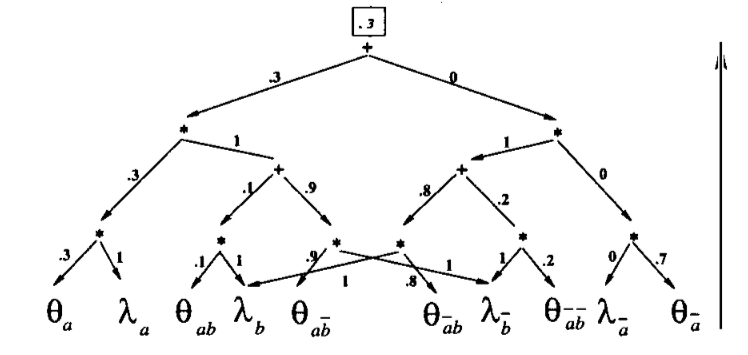
\includegraphics[width=\columnwidth]{figures/compiled.png}
		\caption{Upward phase on an AC.}
		\label{fig:comp}
    \end{center}
\end{figure}

Second phase, messages are sent from nodes to children in the same rooted DAG, leading to computation of all partial derivatives.
This process is known as \emph{back propagation} \citep{rumelhart1988learning}, a common method of training artificial neural networks, and its proven to be able to compute the partial derivatives of variables on the leaves.
The phase starts from the root down to the leaves.
The derivative value of the root, by definition, is always 1.
For the remaining nodes $v$, if the parent $Pa(v)$ is a summation node, the derivative value of $v$ is equal to its parent.
If the parent $Pa(v)$ is a multiplication node, the derivative value of $v$ is equal to the summation of its parent times the others siblings of $v$.
This processes is illustrated in Figure \ref{fig:deri}.
Note that the derivative of a node of a node can not be computed before all its parents derivatives has been computed.
Second phase is described in lines 13-27 in Algorithm 35.

\begin{figure}[!htb]
    \begin{center}
    	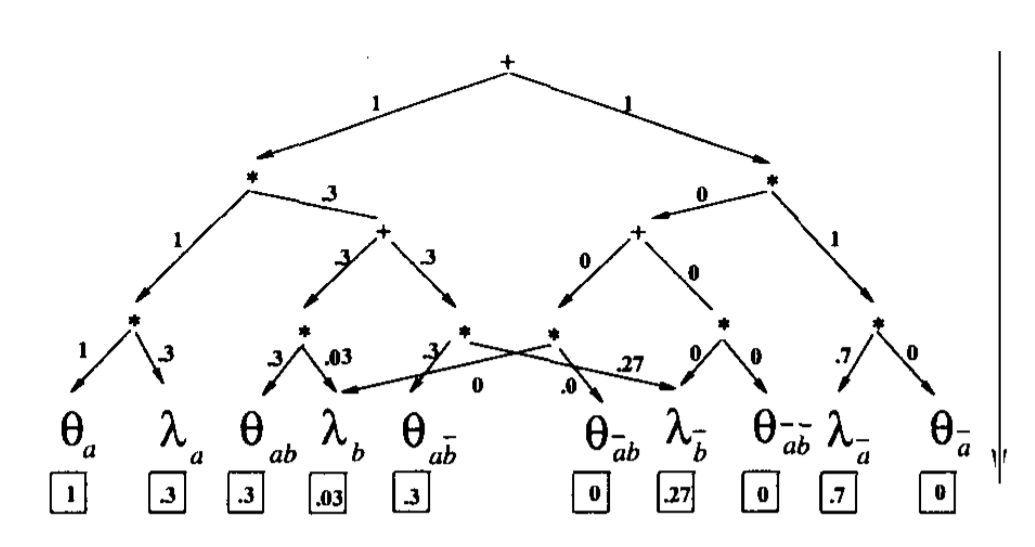
\includegraphics[width=\columnwidth]{figures/deriv.png}
		\caption{Second phase of the evaluation of AC in Figure 5, under evidence $E=A$.}
		\label{fig:deri}
    \end{center}
\end{figure}

\begin{figure}[!htb]
    \begin{center}
    	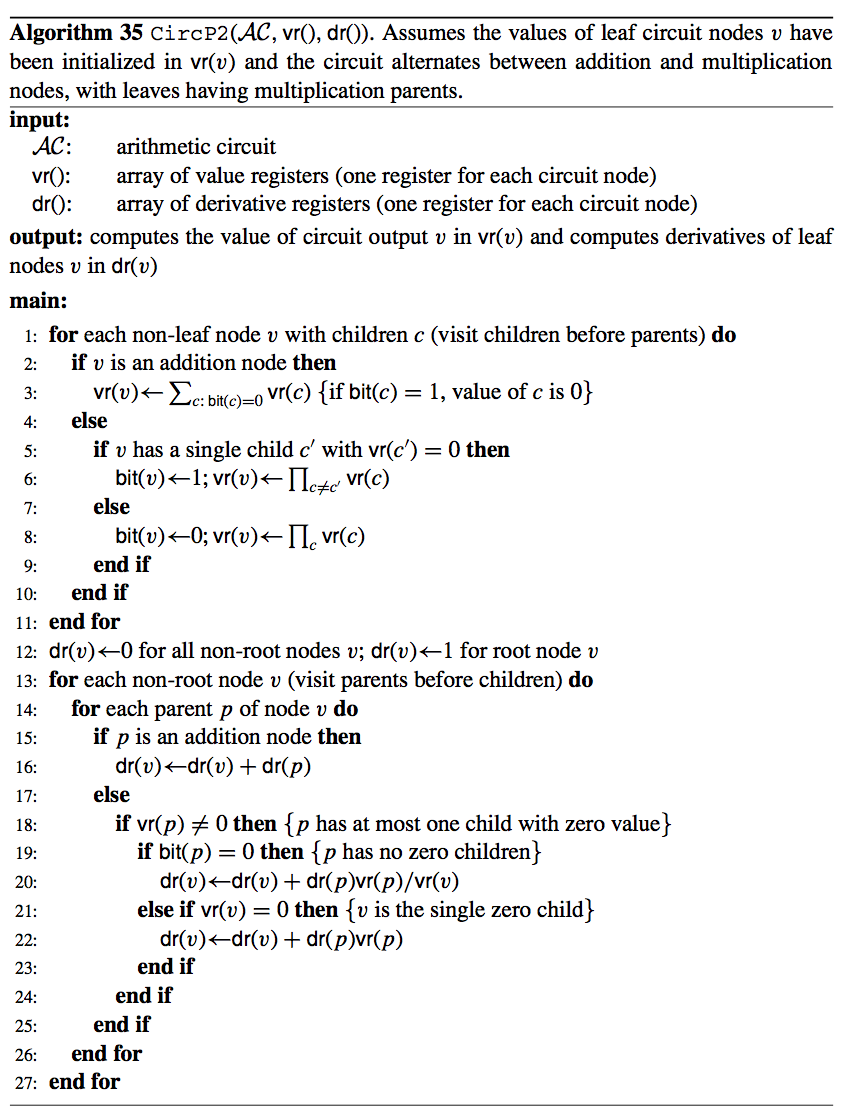
\includegraphics[width=\columnwidth]{figures/alg.png}
%		\caption{}
		\label{fig:alg}
    \end{center}
\end{figure}

After the two-phase steps we have the capacity to answer, in constant time, a very large class of probabilistic queries, relating to classical inference, parameter estimation, model validation and sensitivity analysis.
Some of those queries are
(i) in the root node the probability of the evidence, and 
(ii) the posterior marginal of any network variable.

\subsubsection{Serial Solution}

The serial solution computes the values and derivatives of each node sequentially in both cases.
The only restrictions are those imposed by the topological ordering.
For instance, the second phase where the derivatives are propagated top-bottom, can be implemented with \emph{breadth-first search} algorithm.

\subsubsection{Parallel Solution}

The phases of evaluating and differentiating an AC can improved by the parallelization of the nodes value calculation.
Phase one, massages are sent from nodes to their parents in the AC following the operations of each node, as described in lines 1-11 in Algorithm 1.
Since the phase starts from the leaves up to the root, the layers of operations (sum and product) can be computed in parallel.
For instance, in the second last layer of Figure \ref{fig:comp}, the value of nodes 
($\theta_a \star \lambda_a$), 
($\theta_{ab} \star \lambda_{{b}}$), 
($\theta_{a{\bar b}} \star \lambda_{{\bar b}}$),
($\lambda_{{b}} \star \theta_{{\bar a}b}$),
($\lambda_{{\bar b}} \star \theta_{{\bar a}\bar{b}}$), and
($\lambda_{{\bar a}} \star \theta_{{\bar a}}$) 
can be computed in parallel.


In the second phase, messages are sent from nodes to children in the same rooted DAG, leading to computation of all partial derivatives, as described in lines 12-27 in Algorithm 1.
Since the phase starts from the root down to the leaves, the derivatives of the layers of children can be computed in parallel.
For instance, in the last layers of Figure \ref{fig:deri}, the derivatives of  nodes 
$\theta_a $,
$\lambda_a$,
$\theta_{ab}$,
$\lambda_{{b}}$,
$\theta_{a{\bar b}}$,
$\theta_{{\bar a}b}$,
$\lambda_{{\bar b}}$,
$\theta_{\bar{a}\bar{b}}$,
$\lambda_{{\bar a}}$, and
$\theta_{{\bar a}}$
can be computed in parallel.

\section{Experimental Results}
\label{sec:exp}

ACs are known for been a special case of neural networks \citep{poon2011sum,delalleau2011shallow,peharz2013greedy}.
In fact, the main differences are only (i) the activations functions, which are either sum and products on AC, and (ii) the data is a joint probability distribution.
That been said, we implement a parallel solution for Algorithm 35 using a Python library called \emph{keras} \citep{chollet2015}.
Keras is a modular neural networks library, written in Python, for fast experimentation.


\begin{lstlisting}[language=python]
import numpy as np
from keras.models import Sequential
from keras.layers.core import Dense, Dropout, Layer, Activation
import time
import tensorflow as tf

f = open("results.csv", "w")


INPUT_SIZE = 10
OUTPUT_SIZE = INPUT_SIZE
nb_class = 3

batch_size = 128
nb_epoch = 40

np.random.seed(123)

X_train = np.random.rand(INPUT_SIZE, nb_class)
Y_train = np.random.rand(OUTPUT_SIZE, nb_class)

X_test = np.random.rand(INPUT_SIZE)
Y_test = np.random.rand(OUTPUT_SIZE)

for i in range(1,51):

    start_time = time.time()

    model = Sequential()
    model.add(Dense(INPUT_SIZE, input_shape=(nb_class,)))
    model.add(Activation('linear'))
    model.add(Dense(OUTPUT_SIZE))
    model.add(Activation('linear'))
    model.compile(loss='categorical_crossentropy', optimizer='rmsprop')

    final_time = time.time()
    diff_time = final_time - start_time

    f.write(str(i)+","+str(diff_time)+","+"\n")

f.close() 
\end{lstlisting}
 

We report an empirical comparison between parallel and serial AC compilation solutions.
The experiments were conducted on a 2.9 GHz Intel Core i7 with 8 GB RAM.
The experiments were performed 50 times for each solution.
The total time in seconds required by the parallel and serial solutions are reported in Table \ref{tab:bench_bns}.

From Table \ref{tab:bench_bns}, the implementation of a serial solution is slower than that of d-separation on all runs.
The main reason is that Algorithm 35 can have two parallelizations, the  0first and second phase.
However, note that there are variations on the times reported.
Those variations are due the fact an AC can be constructed in a different manner according to different elimination orderings\footnote{
For more information please check the \href{https://github.com/andreeds/cs807-research-tasks/blob/master/A\%20-\%20The\%20Paper/Paper/Task_A_Andre_200334126.pdf}{Task A - \emph{The Paper} PDF paper}}.

 
 
\begin{table}[!h]
	\begin{center}
	\caption{Comparison of parallel and serial solutions for ACs with 50 runs each}
%	  \resizebox{\columnwidth}{!}{
	  \begin{tabular}{ l | cc }
Solution & Time average & Standard deviation \\ \hline
Serial		& 	0.1610		&	0.0536	\\
Parallel 	& 	0.0434		&	0.0082
		\label{tab:bench_bns}
	\end{tabular}
%	}
  	\end{center}
\end{table}

\begin{figure}[H]
    \begin{center}
    	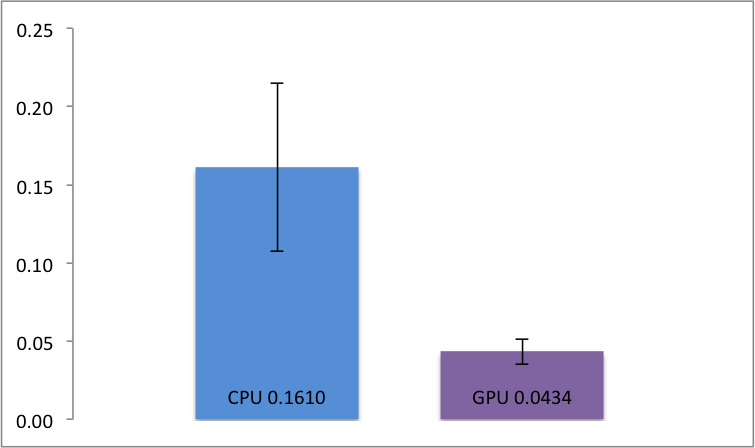
\includegraphics[width=0.7\columnwidth]{figures/graph.png}
		\caption{Comparison between CPU and GPU implementation of AC compiling.}
		\label{fig:deri}
    \end{center}
\end{figure}

\section{Conclusion}
\label{sec:conc}

Reasoning with ACs presents several advantages.
It emphasizes the role of partial differentiation on probabilistic reasoning, giving a new utility to central tasks of BNs.
Also, it helps the migration of BN applications to embedded systems, which are known for constraint in computational resources.


There are two phases to compile the AC: upward and inward.
In this paper we presented the algorithm to compile the AC, drawn from \cite{darwiche2009modeling}.
We have implemented a parallel solution and compared to a serial solution.
Our experimental results indicate that the parallel solution is especially effective in ACs.
However, different elimination ordering of variables upon the construction of the AC can influence on the compilation time.

\vskip 0.2in
\bibliography{references/references}
\end{document}
